\documentclass[12pt,a4paper]{article}

% ─── Page Layout ───────────────────────────────────────────────────────────────
\usepackage[a4paper, margin=0.8in, headheight=14pt]{geometry}

% ─── Fonts (XeLaTeX) ───────────────────────────────────────────────────────────
\usepackage{fontspec}
\usepackage{unicode-math}
\setmainfont{TeX Gyre Pagella}
\setmonofont[Scale=0.88]{TeX Gyre Cursor}
\setmathfont{Latin Modern Math}

% ─── Packages ──────────────────────────────────────────────────────────────────
\usepackage{xcolor}
\usepackage{colortbl}
\usepackage{titlesec}
\usepackage{enumitem}
\usepackage{tabularx}
\usepackage{booktabs}
\usepackage{array}
\usepackage{amsmath}
\usepackage{tikz}
\usetikzlibrary{shapes.geometric, arrows.meta, positioning, calc, fit, decorations.pathreplacing, patterns}
\usepackage{tcolorbox}
\tcbuselibrary{skins, breakable}
\usepackage{hyperref}
\usepackage{fancyhdr}
\usepackage{graphicx}
\usepackage{microtype}
\hyphenpenalty=10000
\exhyphenpenalty=10000
\sloppy
\usepackage{caption}
\usepackage{setspace}
\usepackage{multirow}
\usepackage{tocloft}

% ─── Q&A helper ────────────────────────────────────────────────────────────────
\newcommand{\Q}[1]{\textbf{#1}\par\noindent\ignorespaces}

% ─── Colour Palette ────────────────────────────────────────────────────────────
\definecolor{myred}{RGB}{196,30,58}
\definecolor{mydark}{RGB}{30,30,50}
\definecolor{mygreen}{RGB}{14,120,80}
\definecolor{myteal}{RGB}{0,130,140}
\definecolor{myamber}{RGB}{180,100,0}
\definecolor{mypurple}{RGB}{100,30,160}
\definecolor{mygray}{RGB}{246,247,249}
\definecolor{mgframe}{RGB}{180,185,200}
\definecolor{watermark}{RGB}{145,150,170}
\definecolor{hdrred}{RGB}{250,232,235}
\definecolor{hdrgreen}{RGB}{220,244,233}
\definecolor{hdrteal}{RGB}{220,242,244}
\definecolor{hdramber}{RGB}{253,242,215}
\definecolor{hdrpurple}{RGB}{238,228,255}
\definecolor{hdrgray}{RGB}{238,240,245}
\definecolor{rowalt}{RGB}{250,251,253}

% ─── Section Formatting ────────────────────────────────────────────────────────
\titleformat{\section}
  {\large\bfseries\color{myred}}{\thesection.}{0.5em}{}
  [\vspace{1pt}{\color{myred}\rule{\linewidth}{0.8pt}}]
\titleformat{\subsection}
  {\normalsize\bfseries\color{myteal}}{\thesubsection}{0.5em}{}
\titlespacing*{\section}{0pt}{18pt}{7pt}
\titlespacing*{\subsection}{0pt}{11pt}{4pt}

% ─── Paragraph ─────────────────────────────────────────────────────────────────
\setlength{\parindent}{0pt}
\setlength{\parskip}{4pt}

% ─── TOC Styling ───────────────────────────────────────────────────────────────
\renewcommand{\cfttoctitlefont}{\large\bfseries\color{myred}}
\renewcommand{\cftaftertoctitle}{\par\noindent{\color{myred}\rule{\linewidth}{0.8pt}}}
\setlength{\cftbeforetoctitleskip}{0pt}
\setlength{\cftaftertoctitleskip}{6pt}
\renewcommand{\cftsecfont}{\normalsize\bfseries\color{mydark}}
\renewcommand{\cftsecpagefont}{\normalsize\bfseries\color{mydark}}
\renewcommand{\cftsecleader}{\cftdotfill{\cftdotsep}}
\setlength{\cftbeforesecskip}{7pt}
\renewcommand{\cftsubsecfont}{\small\color{mydark}}
\renewcommand{\cftsubsecpagefont}{\small\color{mydark}}
\setlength{\cftbeforesubsecskip}{3pt}
\setlength{\cftsubsecindent}{1.4em}

% ─── Table helpers ─────────────────────────────────────────────────────────────
\renewcommand{\arraystretch}{1.45}
\setlength{\tabcolsep}{6pt}
\arrayrulecolor{mydark}
\newcolumntype{B}[1]{>{\small\bfseries\raggedright\arraybackslash}m{#1}}
\newcolumntype{Y}{>{\small\raggedright\arraybackslash}X}
\renewcommand{\tabularxcolumn}[1]{m{#1}}

% ─── Header / Footer ───────────────────────────────────────────────────────────
\pagestyle{fancy}
\fancyhf{}
\fancyhead[L]{\small\color{myred}\textbf{EC402}\;\color{mydark}--- Analog Circuits}
\fancyhead[R]{\small\color{myteal}\textbf{Module 4 Notes}}
\fancyfoot[C]{\small\color{mydark}\thepage}
\fancyfoot[R]{\small\color{watermark}\textit{\copyright\ Biraj}}
\renewcommand{\headrulewidth}{0.5pt}
\renewcommand{\footrulewidth}{0.3pt}

% ─── Hyperref ──────────────────────────────────────────────────────────────────
\hypersetup{
  colorlinks=true, linkcolor=myteal, urlcolor=myteal,
  pdfauthor={Biraj Sarkar (CGEC)},
  pdftitle={EC402 --- Module 4 Notes: Differential Amplifiers, Op-Amps and Active Filters}
}

% ─── tcolorbox styles ──────────────────────────────────────────────────────────
\tcbset{
  tikzbox/.style={
    colback=mygray, colframe=mgframe, boxrule=0.6pt, arc=4pt,
    left=8pt, right=8pt, top=6pt, bottom=6pt,
    colbacktitle=mgframe, coltitle=mydark, fonttitle=\small\bfseries
  },
  defbox/.style={
    colback=hdrgreen, colframe=mygreen, boxrule=0.8pt, arc=4pt,
    left=9pt, right=9pt, top=6pt, bottom=6pt,
    colbacktitle=mygreen, coltitle=white, fonttitle=\small\bfseries
  },
  formulabox/.style={
    colback=hdrteal, colframe=myteal, boxrule=0.8pt, arc=4pt,
    left=9pt, right=9pt, top=7pt, bottom=7pt,
    colbacktitle=myteal, coltitle=white, fonttitle=\small\bfseries
  },
  examplebox/.style={
    colback=hdramber, colframe=myamber, boxrule=0.8pt, arc=4pt,
    left=9pt, right=9pt, top=6pt, bottom=6pt,
    colbacktitle=myamber, coltitle=white, fonttitle=\small\bfseries
  },
  masonbox/.style={
    colback=hdrpurple, colframe=mypurple, boxrule=0.8pt, arc=4pt,
    left=9pt, right=9pt, top=6pt, bottom=6pt,
    colbacktitle=mypurple, coltitle=white, fonttitle=\small\bfseries
  },
  exambox/.style={
    colback=hdrpurple, colframe=mypurple, boxrule=1pt, arc=5pt,
    left=10pt, right=10pt, top=8pt, bottom=8pt,
    colbacktitle=mypurple, coltitle=white, fonttitle=\bfseries,
    breakable, title after break={\textbf{Frequently Asked / Viva Questions (contd.)}}
  }
}
\tcbset{breakable}
\tcbset{after={\color{black}}}

% ─── TikZ styles ───────────────────────────────────────────────────────────────
\tikzset{
  block/.style={rectangle, draw=myteal, fill=hdrteal,
    text width=2.4cm, align=center, minimum height=0.95cm,
    font=\small, rounded corners=3pt, line width=0.7pt},
  redblock/.style={rectangle, draw=myred, fill=hdrred,
    text width=2.4cm, align=center, minimum height=0.95cm,
    font=\small, rounded corners=3pt, line width=0.7pt},
  sumjunc/.style={circle, draw=myamber, fill=hdramber,
    minimum size=0.62cm, font=\small, line width=0.8pt},
  arrow/.style={-Stealth, thick, color=mydark},
  redarrow/.style={-Stealth, thick, color=myred},
  line/.style={thick, color=mydark}
}

\begin{document}

% ─── Title Page ───────────────────────────────────────────────────────────────
\begin{center}
  {\LARGE\bfseries\color{myred} EC402 --- Analog Circuits}\\[5pt]
  {\normalsize\color{mydark} Semester IV \quad$\bullet$\quad 3L:0T:0P \quad$\bullet$\quad 3 Credits}\\[3pt]
  {\normalsize\color{myteal}\textbf{Module 4 Exam Notes: Differential Amplifiers, Op-Amps and Active Filters}}\\[3pt]
  {\small\color{mydark} CGEC \;$|$\; B.Tech ECE (2023--27) \;$|$\; \textit{Biraj Sarkar}}
\end{center}
\vspace{-2pt}
\noindent\rule{\linewidth}{0.8pt}
\vspace{-2pt}

\begin{tcolorbox}[defbox, title={Module Scope \& Key Learning Objectives}]
Module 4 explores the backbone of analog and mixed-signal instrumentation:
\begin{itemize}[leftmargin=12pt, itemsep=2pt, topsep=1pt]
  \item \textbf{Differential Amplifiers}: Emitter-coupled pairs, half-circuit analysis, differential gain ($A_d$), common-mode gain ($A_c$), Common Mode Rejection Ratio ($\text{CMRR}$), Input Common-Mode Range ($\text{ICMR}$), active load current mirror topology.
  \item \textbf{Operational Amplifiers (Op-Amps)}: Internal architecture (4-stage block diagram), ideal vs. practical characteristics (IC 741), virtual ground concept, inverting and non-inverting configurations.
  \item \textbf{Op-Amp Applications}: Summing amplifiers, 3-op-amp instrumentation amplifiers, lossy integrators, practical differentiators, Log/Anti-log multipliers, Schmitt triggers with hysteresis.
  \item \textbf{Active Filters}: 1st and 2nd-order Sallen-Key low-pass and high-pass filters, Multiple-Feedback (MFB) band-pass filters, Twin-T notch filters, Butterworth pole approximations, and component scaling rules.
\end{itemize}
\end{tcolorbox}

\tableofcontents
\newpage

% ─── Section 1: Differential Amplifier ─────────────────────────────────────────
\section{BJT Differential Amplifier}

\begin{tcolorbox}[defbox, title={Definition: Differential Amplifier}]
A \textbf{Differential Amplifier} is a direct-coupled circuit consisting of two matched transistors configured to amplify the algebraic difference between two input signals while attenuating any signal common to both inputs. It forms the essential input stage of operational amplifiers and linear integrated circuits.
\end{tcolorbox}

\subsection{Basic Architecture and Principle of Operation}
The basic emitter-coupled differential amplifier consists of two matched transistors ($Q_1, Q_2$), identical collector resistors $R_{C1} = R_{C2} = R_C$, and an emitter resistance $R_E$ (or an active constant current source $I_{EE}$) connected to negative supply $-V_{EE}$.

\begin{tcolorbox}[tikzbox, title={BJT Emitter-Coupled Differential Pair Architecture}]
\centering
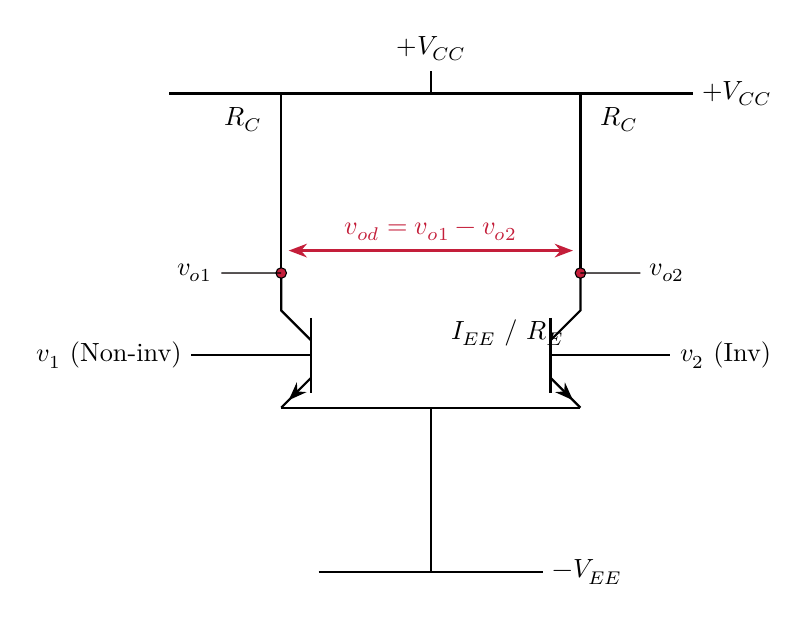
\begin{tikzpicture}[scale=0.95, transform shape]
  % VCC rail
  \draw[thick] (-3.5, 3.2) -- (3.5, 3.2) node[right] {$+V_{CC}$};
  \draw[thick] (0, 3.2) -- (0, 3.5) node[above] {$+V_{CC}$};

  % Resistors RC1, RC2
  \draw[thick] (-2, 3.2) -- (-2, 2.5) to[rectangle, draw=myteal, fill=hdrteal, minimum width=0.6cm, minimum height=1cm] (-2, 1.5) node[midway, left=4pt] {$R_C$} -- (-2, 0.8);
  \draw[thick] (2, 3.2) -- (2, 2.5) to[rectangle, draw=myteal, fill=hdrteal, minimum width=0.6cm, minimum height=1cm] (2, 1.5) node[midway, right=4pt] {$R_C$} -- (2, 0.8);

  % Transistors Q1 and Q2
  \draw[thick] (-2, 0.8) -- (-2, 0.3) -- (-1.6, -0.1); % Collector Q1
  \draw[thick] (-1.6, -0.6) -- (-2, -1.0); % Emitter Q1
  \draw[thick, -Stealth] (-1.8, -0.8) -- (-1.9, -0.9);
  \draw[thick] (-1.6, 0.2) -- (-1.6, -0.8); % Base bar Q1
  \draw[thick] (-1.6, -0.3) -- (-3.2, -0.3) node[left] {$v_1$ (Non-inv)};

  \draw[thick] (2, 0.8) -- (2, 0.3) -- (1.6, -0.1); % Collector Q2
  \draw[thick] (1.6, -0.6) -- (2, -1.0); % Emitter Q2
  \draw[thick, -Stealth] (1.8, -0.8) -- (1.9, -0.9);
  \draw[thick] (1.6, 0.2) -- (1.6, -0.8); % Base bar Q2
  \draw[thick] (1.6, -0.3) -- (3.2, -0.3) node[right] {$v_2$ (Inv)};

  % Common Emitter connection
  \draw[thick] (-2, -1.0) -- (0, -1.0) -- (2, -1.0);
  \draw[thick] (0, -1.0) -- (0, -1.6);

  % Tail current source / RE
  \draw[thick] (0, -1.6) to[rectangle, draw=myamber, fill=hdramber, minimum width=0.7cm, minimum height=1.1cm] (0, -2.7) node[midway, right=4pt] {$I_{EE}$ / $R_E$} -- (0, -3.2);
  \draw[thick] (-1.5, -3.2) -- (1.5, -3.2) node[right] {$-V_{EE}$};

  % Output nodes
  \draw[fill=myred] (-2, 0.8) circle (2pt) -- (-2.8, 0.8) node[left] {$v_{o1}$};
  \draw[fill=myred] (2, 0.8) circle (2pt) -- (2.8, 0.8) node[right] {$v_{o2}$};
  \draw[thick, Stealth-Stealth, color=myred] (-1.9, 1.1) -- (1.9, 1.1) node[midway, above] {$v_{od} = v_{o1} - v_{o2}$};
\end{tikzpicture}
\end{tcolorbox}

\subsection{Large-Signal Transfer Characteristics}
Assuming active region operation where $I_C \approx I_E = I_S e^{V_{BE}/V_T}$:
\begin{align}
  v_1 - v_2 &= v_{id} = V_{BE1} - V_{BE2} = V_T \ln\left(\frac{I_{C1}}{I_{C2}}\right) \\
  \frac{I_{C1}}{I_{C2}} &= e^{v_{id}/V_T}
\end{align}
Since $I_{C1} + I_{C2} = I_{EE}$ (neglecting base currents):
\begin{tcolorbox}[formulabox, title={Large-Signal Differential Collector Currents}]
\begin{equation}
  I_{C1} = \frac{I_{EE}}{1 + e^{-v_{id}/V_T}}, \qquad I_{C2} = \frac{I_{EE}}{1 + e^{v_{id}/V_T}}
\end{equation}
The output differential voltage is:
\begin{equation}
  v_{od} = v_{o1} - v_{o2} = -(I_{C1} - I_{C2})R_C = -I_{EE} R_C \tanh\left(\frac{v_{id}}{2V_T}\right)
\end{equation}
\end{tcolorbox}
\textbf{Linear Range}: For small inputs $|v_{id}| < 2V_T \approx 50\text{ mV}$, $\tanh(x) \approx x$. When $|v_{id}| \ge 4V_T \approx 100\text{ mV}$, current completely steers into one transistor, causing hard saturation/clipping.

\subsection{Small-Signal Half-Circuit Analysis}
Any pair of arbitrary input voltages $v_1, v_2$ can be decomposed into:
\begin{equation}
  v_{id} = v_1 - v_2 \quad (\text{Differential Mode}), \qquad v_{icm} = \frac{v_1 + v_2}{2} \quad (\text{Common Mode})
\end{equation}
such that $v_1 = v_{icm} + \frac{v_{id}}{2}$ and $v_2 = v_{icm} - \frac{v_{id}}{2}$.

\subsubsection{Differential-Mode Half Circuit}
When $v_1 = +v_{id}/2$ and $v_2 = -v_{id}/2$, the circuit exhibits anti-symmetry. The common emitter node potential remains constant at $0\text{ V}$ (virtual ground for differential signals). The tail impedance $R_E$ carries zero signal current:
\begin{tcolorbox}[formulabox, title={Differential Gain ($A_d$) \& Input Impedance ($R_{id}$)}]
\begin{equation}
  A_d = \frac{v_{o1} - v_{o2}}{v_1 - v_2} = -g_m R_C = -\frac{I_{EE} R_C}{2 V_T}
\end{equation}
For single-ended output ($v_o = v_{o1}$):
\begin{equation}
  A_{d,\text{single}} = -\frac{1}{2} g_m R_C
\end{equation}
Differential input resistance:
\begin{equation}
  R_{id} = 2 r_\pi = 2\,\frac{\beta}{g_m} = 4\,\frac{\beta V_T}{I_{EE}}
\end{equation}
\end{tcolorbox}

\subsubsection{Common-Mode Half Circuit}
When $v_1 = v_2 = v_{icm}$, both halves conduct equally in parallel. The tail resistor $R_E$ splits into two parallel resistors of value $2R_E$:
\begin{tcolorbox}[formulabox, title={Common-Mode Gain ($A_c$) \& Input Impedance ($R_{icm}$)}]
\begin{equation}
  A_c = \frac{v_{ocm}}{v_{icm}} = -\frac{g_m R_C}{1 + 2 g_m R_E} \approx -\frac{R_C}{2 R_E} \quad (\text{for } 2g_m R_E \gg 1)
\end{equation}
Common-mode input resistance:
\begin{equation}
  R_{icm} = r_\pi + 2(1+\beta)R_E \approx 2\beta R_E
\end{equation}
\end{tcolorbox}

\subsection{Common-Mode Rejection Ratio (CMRR)}
\begin{tcolorbox}[defbox, title={Common Mode Rejection Ratio}]
\textbf{CMRR} measures the ability of a differential amplifier to reject common-mode noise and amplify only the differential signal:
\begin{equation}
  \text{CMRR} = \left|\frac{A_d}{A_c}\right| = \frac{g_m R_C}{\frac{g_m R_C}{1 + 2g_m R_E}} = 1 + 2g_m R_E \approx 2 g_m R_E = \frac{I_{EE} R_E}{V_T}
\end{equation}
Expressed in decibels:
\begin{equation}
  \text{CMRR}_{\text{dB}} = 20 \log_{10}\left|\frac{A_d}{A_c}\right|
\end{equation}
\end{tcolorbox}
\textbf{Design Implication}: To maximize CMRR, $R_E$ must be made arbitrarily large. In modern IC design, $R_E$ is replaced by an active BJT/MOSFET current mirror, providing incremental output resistance $r_o$ in the megaohm range, pushing CMRR well above $100\text{ dB}$.

\subsection{Input Common-Mode Range (ICMR)}
\begin{tcolorbox}[formulabox, title={Input Common-Mode Range Boundaries}]
$\text{ICMR}$ is the allowable range of common-mode input voltage $v_{icm}$ for which all transistors remain in the active region:
\begin{align}
  V_{icm,\max} &= V_{CC} - I_C R_C + V_{BE} = V_{CC} - \frac{I_{EE} R_C}{2} + 0.7\text{ V} \\
  V_{icm,\min} &= -V_{EE} + V_{CS} + V_{BE}
\end{align}
where $V_{CS}$ is the minimum compliance voltage required across the tail current source to avoid saturation ($\approx 0.3\text{ V}$ for BJT, $V_{ov}$ for MOSFET).
\end{tcolorbox}

% ─── Section 2: Operational Amplifiers ─────────────────────────────────────────
\section{Operational Amplifier (Op-Amp) Fundamentals}

\begin{tcolorbox}[defbox, title={Definition: Operational Amplifier}]
An \textbf{Operational Amplifier (Op-Amp)} is a direct-coupled, high-gain integrated voltage amplifier with differential inputs and single-ended output, designed to perform linear and non-linear mathematical operations via negative and positive feedback networks.
\end{tcolorbox}

\subsection{Internal Architecture: 4-Stage Block Diagram}
\begin{tcolorbox}[tikzbox, title={Internal Block Diagram of Modern IC Op-Amp}]
\centering
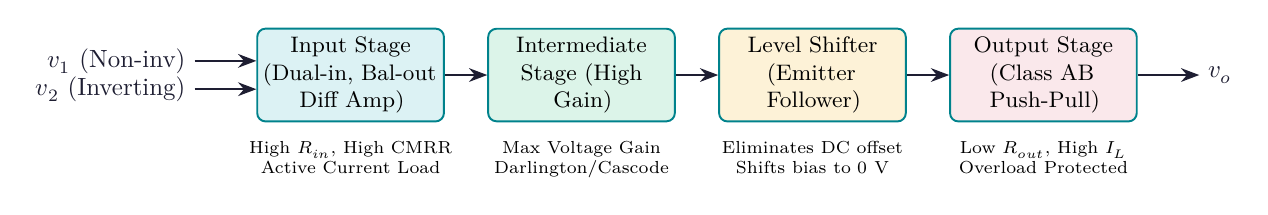
\begin{tikzpicture}[scale=0.9, transform shape, node distance=0.6cm]
  \node[block, fill=hdrteal] (in) {Input Stage\\(Dual-in, Bal-out Diff Amp)};
  \node[block, right=of in, fill=hdrgreen] (inter) {Intermediate\\Stage (High Gain)};
  \node[block, right=of inter, fill=hdramber] (level) {Level Shifter\\(Emitter Follower)};
  \node[block, right=of level, fill=hdrred] (out) {Output Stage\\(Class AB Push-Pull)};

  \draw[arrow] (-2.2, 0.2) node[left] {$v_1$ (Non-inv)} -- (in.west |- 0, 0.2);
  \draw[arrow] (-2.2, -0.2) node[left] {$v_2$ (Inverting)} -- (in.west |- 0, -0.2);
  \draw[arrow] (in) -- (inter);
  \draw[arrow] (inter) -- (level);
  \draw[arrow] (level) -- (out);
  \draw[arrow] (out) -- ++(2.2, 0) node[right] {$v_o$};

  \node[below=0.15cm of in, font=\scriptsize, align=center] {High $R_{in}$, High CMRR\\Active Current Load};
  \node[below=0.15cm of inter, font=\scriptsize, align=center] {Max Voltage Gain\\Darlington/Cascode};
  \node[below=0.15cm of level, font=\scriptsize, align=center] {Eliminates DC offset\\Shifts bias to $0\text{ V}$};
  \node[below=0.15cm of out, font=\scriptsize, align=center] {Low $R_{out}$, High $I_L$\\Overload Protected};
\end{tikzpicture}
\end{tcolorbox}

\subsection{Ideal vs. Practical Op-Amp Characteristics (IC 741)}
\par\vspace{6pt}\noindent
\begin{tabularx}{\linewidth}{|B{3.4cm}|Y|Y|B{3.2cm}|}
\hline
\textbf{Parameter} & \textbf{Ideal Value} & \textbf{Typical IC 741} & \textbf{Significance} \\
\hline
Open-Loop Voltage Gain ($A_{OL}$) & $\infty$ & $2 \times 10^5$ ($106\text{ dB}$) & Eliminates gain error \\
Input Resistance ($R_{in}$) & $\infty$ & $2\text{ M}\Omega$ (FET: $> 10^{12}\Omega$) & Eliminates source loading \\
Output Resistance ($R_{out}$) & $0\,\Omega$ & $75\,\Omega$ & Zero loading by load $R_L$ \\
Bandwidth ($\text{BW}$) & $\infty$ & $1\text{ MHz}$ (Unity GBW) & Constant gain across frequency \\
CMRR & $\infty$ & $90\text{ dB}$ & Rejects common-mode noise \\
Slew Rate ($\text{SR}$) & $\infty$ & $0.5\text{ V}/\mu\text{s}$ & Maximum rate of output swing \\
Input Offset Voltage ($V_{ios}$) & $0\text{ V}$ & $2\text{ mV}$ & DC voltage mismatch at input \\
Input Bias Current ($I_B$) & $0\text{ A}$ & $80\text{ nA}$ & Average DC base currents \\
Input Offset Current ($I_{ios}$) & $0\text{ A}$ & $20\text{ nA}$ & Difference between base currents \\
\hline
\end{tabularx}
\vspace{12pt}

\subsection{Slew Rate and Full-Power Bandwidth}
\begin{tcolorbox}[formulabox, title={Slew Rate and Maximum Frequency Formulation}]
\textbf{Slew Rate (SR)} is the maximum rate of change of output voltage that the op-amp can deliver under large-signal step excitation, limited by the charging of internal compensation capacitor $C_c$:
\begin{equation}
  \text{SR} = \left.\frac{dv_o}{dt}\right|_{\max} = \frac{I_{EE}}{C_c} \quad [\text{V}/\mu\text{s}]
\end{equation}
For an undistorted output sinusoid $v_o(t) = V_m \sin(2\pi f t)$:
\begin{equation}
  \left.\frac{dv_o}{dt}\right|_{\max} = 2\pi f V_m \le \text{SR} \implies f_{\max} = \frac{\text{SR}}{2\pi V_m}
\end{equation}
where $f_{\max}$ is the \textbf{Full-Power Bandwidth}. If input frequency exceeds $f_{\max}$, the output degenerates from a sine wave into a slew-limited triangular wave.
\end{tcolorbox}

\subsection{Basic Inverting and Non-Inverting Configurations}

\begin{tcolorbox}[tikzbox, title={Fundamental Inverting and Non-Inverting Op-Amp Topologies}]
\centering
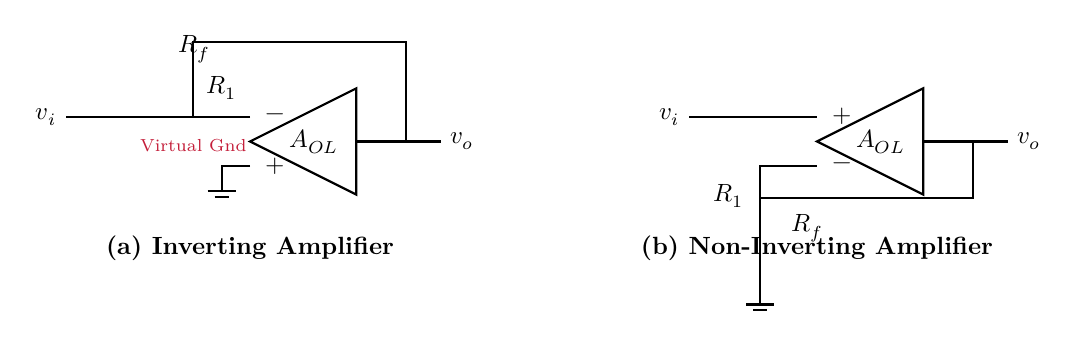
\begin{tikzpicture}[scale=0.9, transform shape]
  % Inverting Amplifier
  \begin{scope}[shift={(-4.2,0)}]
    \draw[thick] (0, 0) -- (1.5, 0.75) -- (1.5, -0.75) -- cycle; % Opamp triangle
    \node at (0.35, 0.35) {$-$};
    \node at (0.35, -0.35) {$+$};
    \node at (0.9, 0) {$A_{OL}$};

    % Inputs
    \draw[thick] (0, 0.35) -- (-0.8, 0.35) to[rectangle, draw=myteal, fill=hdrteal, minimum width=0.8cm, minimum height=0.4cm] (-1.8, 0.35) node[midway, above=3pt] {$R_1$} -- (-2.6, 0.35) node[left] {$v_i$};
    \draw[thick] (0, -0.35) -- (-0.4, -0.35) -- (-0.4, -0.7);
    \draw[thick] (-0.6, -0.7) -- (-0.2, -0.7);
    \draw[thick] (-0.5, -0.78) -- (-0.3, -0.78);

    % Feedback Rf
    \draw[thick] (-0.8, 0.35) -- (-0.8, 1.4) to[rectangle, draw=myteal, fill=hdrteal, minimum width=0.8cm, minimum height=0.4cm] (0.8, 1.4) node[midway, above=3pt] {$R_f$} -- (2.2, 1.4) -- (2.2, 0);

    % Output
    \draw[thick] (1.5, 0) -- (2.7, 0) node[right] {$v_o$};
    \node at (-0.8, 0.15) [below, font=\scriptsize, color=myred] {Virtual Gnd};
    \node at (0, -1.5) [font=\bfseries] {(a) Inverting Amplifier};
  \end{scope}

  % Non-Inverting Amplifier
  \begin{scope}[shift={(3.8,0)}]
    \draw[thick] (0, 0) -- (1.5, 0.75) -- (1.5, -0.75) -- cycle;
    \node at (0.35, 0.35) {$+$};
    \node at (0.35, -0.35) {$-$};
    \node at (0.9, 0) {$A_{OL}$};

    % Input to Non-inv
    \draw[thick] (0, 0.35) -- (-1.8, 0.35) node[left] {$v_i$};

    % Feedback to Inv
    \draw[thick] (0, -0.35) -- (-0.8, -0.35) -- (-0.8, -1.2) to[rectangle, draw=myteal, fill=hdrteal, minimum width=0.4cm, minimum height=0.8cm] (-0.8, -2.0) node[midway, left=3pt] {$R_1$} -- (-0.8, -2.3);
    \draw[thick] (-1.0, -2.3) -- (-0.6, -2.3);
    \draw[thick] (-0.9, -2.38) -- (-0.7, -2.38);

    \draw[thick] (-0.8, -0.35) -- (-0.8, -0.8) -- (0.5, -0.8) to[rectangle, draw=myteal, fill=hdrteal, minimum width=0.8cm, minimum height=0.4cm] (1.5, -0.8) node[midway, below=3pt] {$R_f$} -- (2.2, -0.8) -- (2.2, 0);

    % Output
    \draw[thick] (1.5, 0) -- (2.7, 0) node[right] {$v_o$};
    \node at (0, -1.5) [font=\bfseries] {(b) Non-Inverting Amplifier};
  \end{scope}
\end{tikzpicture}
\end{tcolorbox}

\begin{tcolorbox}[formulabox, title={Inverting \& Non-Inverting Gain Derivations}]
\textbf{Inverting Configuration}:
By virtual ground ($v_- = v_+ = 0\text{ V}$) and $i_- = 0$:
\begin{equation}
  \frac{v_i - 0}{R_1} + \frac{v_o - 0}{R_f} = 0 \implies A_v = \frac{v_o}{v_i} = -\frac{R_f}{R_1}, \qquad R_{in} = R_1
\end{equation}
\textbf{Non-Inverting Configuration}:
By virtual short ($v_- = v_+ = v_i$) and voltage divider across feedback network:
\begin{equation}
  v_- = v_o \left(\frac{R_1}{R_1 + R_f}\right) = v_i \implies A_v = \frac{v_o}{v_i} = 1 + \frac{R_f}{R_1}, \qquad R_{in} \to \infty
\end{equation}
\textbf{Voltage Follower (Buffer)}: When $R_f = 0$ and $R_1 \to \infty$, $A_v = 1$, $R_{in} \approx \infty$, $R_{out} \approx 0$.
\end{tcolorbox}

% ─── Section 3: Op-Amp Applications ───────────────────────────────────────────
\section{Linear and Non-Linear Op-Amp Applications}

\subsection{Summing Amplifier}
An inverting adder sums multiple weighted input voltages at the virtual ground node:
\begin{equation}
  v_o = -\left(\frac{R_f}{R_1} v_1 + \frac{R_f}{R_2} v_2 + \frac{R_f}{R_3} v_3\right)
\end{equation}
If $R_1 = R_2 = R_3 = R$, then $v_o = -\frac{R_f}{R}(v_1 + v_2 + v_3)$. When $R_f = R/3$, the circuit acts as an analog averager.

\subsection{Three Op-Amp Instrumentation Amplifier}
\begin{tcolorbox}[defbox, title={Three Op-Amp Instrumentation Amplifier}]
The standard 3-op-amp instrumentation amplifier provides ultra-high differential input impedance, high CMRR, and user-variable gain controlled by a single resistor $R_G$.
\end{tcolorbox}

\begin{tcolorbox}[tikzbox, title={Schematic of 3-Op-Amp Instrumentation Amplifier}]
\centering
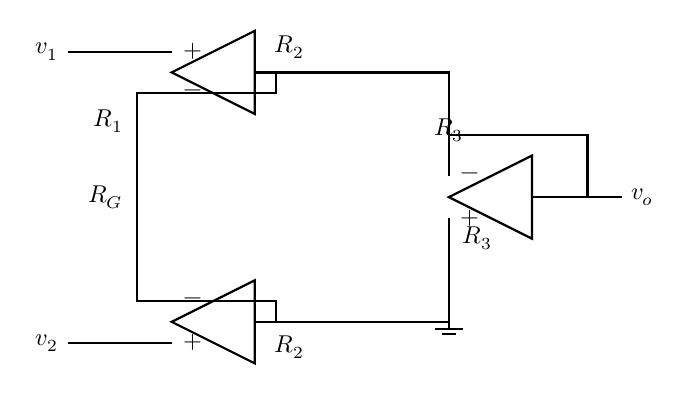
\begin{tikzpicture}[scale=0.88, transform shape]
  % Input Opamp A1
  \draw[thick] (0, 1.8) -- (1.2, 2.4) -- (1.2, 1.2) -- cycle;
  \node at (0.3, 2.1) {$+$}; \node at (0.3, 1.5) {$-$};
  \draw[thick] (0, 2.1) -- (-1.5, 2.1) node[left] {$v_1$};

  % Input Opamp A2
  \draw[thick] (0, -1.8) -- (1.2, -1.2) -- (1.2, -2.4) -- cycle;
  \node at (0.3, -2.1) {$+$}; \node at (0.3, -1.5) {$-$};
  \draw[thick] (0, -2.1) -- (-1.5, -2.1) node[left] {$v_2$};

  % Resistors R1, RG, R1
  \draw[thick] (0, 1.5) -- (-0.5, 1.5) -- (-0.5, 0.7) to[rectangle, draw=myteal, fill=hdrteal, minimum width=0.4cm, minimum height=0.7cm] (-0.5, 0.2) node[midway, left=2pt] {$R_1$} -- (-0.5, -0.2) to[rectangle, draw=myred, fill=hdrred, minimum width=0.4cm, minimum height=0.7cm] (-0.5, -0.7) node[midway, left=2pt] {$R_G$} -- (-0.5, -1.5) -- (0, -1.5);
  \draw[thick] (-0.5, 1.5) -- (1.5, 1.5) -- (1.5, 1.8);
  \draw[thick] (-0.5, -1.5) -- (1.5, -1.5) -- (1.5, -1.8);

  % Output Opamp A3
  \draw[thick] (4, 0) -- (5.2, 0.6) -- (5.2, -0.6) -- cycle;
  \node at (4.3, 0.3) {$-$}; \node at (4.3, -0.3) {$+$};

  % Resistors R2, R3
  \draw[thick] (1.2, 1.8) -- (2.2, 1.8) to[rectangle, draw=myteal, fill=hdrteal, minimum width=0.8cm, minimum height=0.4cm] (3.2, 1.8) node[midway, above=2pt] {$R_2$} -- (4, 1.8) -- (4, 0.3);
  \draw[thick] (1.2, -1.8) -- (2.2, -1.8) to[rectangle, draw=myteal, fill=hdrteal, minimum width=0.8cm, minimum height=0.4cm] (3.2, -1.8) node[midway, below=2pt] {$R_2$} -- (4, -1.8) -- (4, -0.3);

  % Feedback and ground resistors R3
  \draw[thick] (4, 0.3) -- (4, 0.9) to[rectangle, draw=myteal, fill=hdrteal, minimum width=0.8cm, minimum height=0.4cm] (5.4, 0.9) node[midway, above=2pt] {$R_3$} -- (6.0, 0.9) -- (6.0, 0);
  \draw[thick] (4, -0.3) -- (4, -0.9) to[rectangle, draw=myteal, fill=hdrteal, minimum width=0.8cm, minimum height=0.4cm] (4, -1.6) node[midway, right=2pt] {$R_3$} -- (4, -1.9);
  \draw[thick] (3.8, -1.9) -- (4.2, -1.9);
  \draw[thick] (3.9, -1.98) -- (4.1, -1.98);

  \draw[thick] (5.2, 0) -- (6.5, 0) node[right] {$v_o$};
\end{tikzpicture}
\end{tcolorbox}

\begin{tcolorbox}[formulabox, title={Instrumentation Amplifier Transfer Characteristic}]
The intermediate outputs from input buffers $A_1$ and $A_2$ are:
\begin{equation}
  v_{o1}' - v_{o2}' = \left(1 + \frac{2 R_1}{R_G}\right)(v_1 - v_2)
\end{equation}
The difference amplifier $A_3$ produces output:
\begin{equation}
  v_o = \frac{R_3}{R_2}(v_{o2}' - v_{o1}') = \left(1 + \frac{2 R_1}{R_G}\right)\frac{R_3}{R_2}(v_2 - v_1)
\end{equation}
\textbf{Key Merits}:
\begin{enumerate}[leftmargin=14pt, itemsep=2pt, topsep=2pt]
  \item Common-mode voltage is amplified by unity in the first stage, while differential voltage is amplified by $\left(1 + \frac{2R_1}{R_G}\right)$, drastically elevating CMRR.
  \item Gain is tuned via single grounded resistor $R_G$ without disturbing circuit symmetry.
\end{enumerate}
\end{tcolorbox}

\subsection{Integrator and Differentiator}

\subsubsection{Ideal vs. Practical (Lossy) Integrator}
In an ideal integrator, feedback resistor $R_f$ is replaced by capacitor $C$:
\begin{equation}
  v_o(t) = -\frac{1}{R_1 C} \int_0^t v_i(\tau)d\tau + v_o(0), \qquad H(s) = -\frac{1}{s R_1 C}
\end{equation}
\textbf{Fatal Limitation}: At DC ($\omega \to 0$), capacitor impedance $|Z_C| \to \infty$. Any slight input offset voltage or bias current is integrated continuously, driving the op-amp into hard DC saturation rail ($+V_{sat}$ or $-V_{sat}$).

\begin{tcolorbox}[formulabox, title={Practical / Lossy Integrator Formulation}]
To stabilize DC gain, a shunt resistor $R_f$ is placed across $C$:
\begin{equation}
  H(s) = -\frac{Z_f(s)}{R_1} = -\frac{R_f \parallel \frac{1}{sC}}{R_1} = -\frac{R_f / R_1}{1 + s R_f C}
\end{equation}
\begin{itemize}[leftmargin=12pt, itemsep=2pt, topsep=1pt]
  \item \textbf{DC Gain}: $A_v(0) = -\frac{R_f}{R_1}$ (finite, stable).
  \item \textbf{Corner Frequency}: $f_a = \frac{1}{2\pi R_f C}$ (3-dB cutoff).
  \item \textbf{True Integration Band}: Operates as a true mathematical integrator for frequencies $f \ge 10 f_a$, where phase angle approaches $-90^\circ$ and gain rolls off at $-20\text{ dB/decade}$.
\end{itemize}
\end{tcolorbox}

\subsubsection{Ideal vs. Practical Differentiator}
In an ideal differentiator, input resistor $R_1$ is replaced by capacitor $C_1$:
\begin{equation}
  v_o(t) = -R_f C_1 \frac{dv_i}{dt}, \qquad H(s) = -s R_f C_1
\end{equation}
\textbf{Fatal Limitation}: Gain $|H(j\omega)| = \omega R_f C_1$ increases linearly with frequency without bound, severely amplifying high-frequency noise and causing high-frequency oscillations.
\begin{tcolorbox}[formulabox, title={Practical Differentiator}]
A small series resistor $R_1$ is added to $C_1$, and a small capacitor $C_f$ is shunted across $R_f$ such that $R_1 C_1 = R_f C_f$:
\begin{equation}
  H(s) = -\frac{s R_f C_1}{(1 + s R_1 C_1)(1 + s R_f C_f)}
\end{equation}
The circuit differentiates only for $f < f_a = \frac{1}{2\pi R_f C_1}$ and acts as an attenuating low-pass filter above $f_b = \frac{1}{2\pi R_1 C_1}$, guaranteeing unconditional stability.
\end{tcolorbox}

\subsection{Logarithmic and Anti-Logarithmic Amplifiers}
\subsubsection{Logarithmic Amplifier}
By exploiting the exponential $I_C\text{--}V_{BE}$ relationship of a BJT placed in the negative feedback path:
\begin{equation}
  I_{C} = I_S \left(e^{V_{BE}/V_T} - 1\right) \approx I_S e^{V_{BE}/V_T} \implies V_{BE} = V_T \ln\left(\frac{I_C}{I_S}\right)
\end{equation}
Since $v_- = 0\text{ V}$ (virtual ground), $I_C = \frac{v_i}{R_1}$ and $v_o = -V_{BE}$:
\begin{tcolorbox}[formulabox, title={Logarithmic Amplifier Output}]
\begin{equation}
  v_o = -V_T \ln\left(\frac{v_i}{I_S R_1}\right)
\end{equation}
\textbf{Temperature Sensitivity}: $V_T = \frac{kT}{q}$ and $I_S$ double every $5^\circ\text{C}$ rise. Precision log amps employ matched dual transistors with an active temperature-compensating divider containing a positive temperature coefficient PTC thermistor.
\end{tcolorbox}

\subsubsection{Anti-Logarithmic (Exponential) Amplifier}
When the BJT is connected at the input and resistor $R_f$ in the feedback loop:
\begin{equation}
  v_o = -R_f I_C = -R_f I_S e^{v_i/V_T}
\end{equation}
\textbf{Applications}: Analog multiplication ($xy = \text{antilog}[\ln x + \ln y]$), analog division ($x/y = \text{antilog}[\ln x - \ln y]$), root extraction, dynamic range compression.

\subsection{Schmitt Trigger and Hysteresis}
\begin{tcolorbox}[defbox, title={Schmitt Trigger}]
A \textbf{Schmitt Trigger} is a bi-stable regenerative comparator that utilizes positive feedback to establish two distinct switching thresholds, creating an intentional deadband (hysteresis) that completely prevents noise-induced false transitions.
\end{tcolorbox}

\begin{tcolorbox}[tikzbox, title={Inverting Schmitt Trigger and Hysteresis Transfer Curve}]
\centering
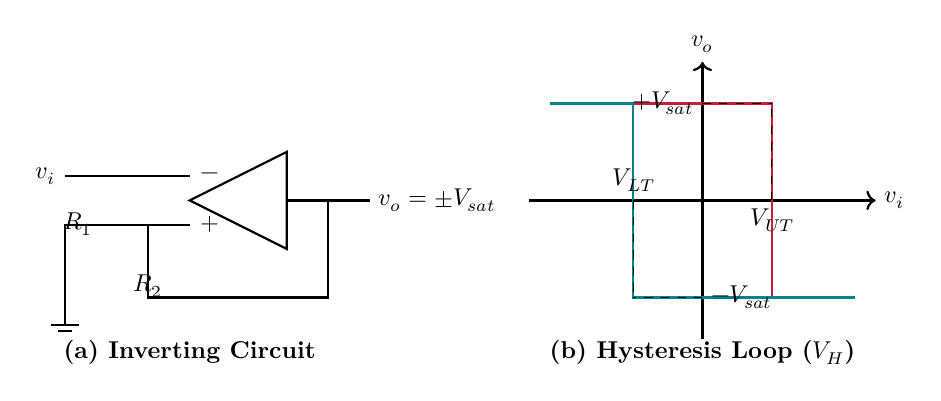
\begin{tikzpicture}[scale=0.88, transform shape]
  % Circuit
  \begin{scope}[shift={(-4.2, 0)}]
    \draw[thick] (0, 0) -- (1.4, 0.7) -- (1.4, -0.7) -- cycle;
    \node at (0.3, 0.35) {$-$}; \node at (0.3, -0.35) {$+$};

    \draw[thick] (0, 0.35) -- (-1.8, 0.35) node[left] {$v_i$};
    \draw[thick] (1.4, 0) -- (2.6, 0) node[right] {$v_o = \pm V_{sat}$};

    % Positive feedback
    \draw[thick] (0, -0.35) -- (-0.6, -0.35) -- (-0.6, -1.4) to[rectangle, draw=myteal, fill=hdrteal, minimum width=0.8cm, minimum height=0.4cm] (0.8, -1.4) node[midway, below=2pt] {$R_2$} -- (2.0, -1.4) -- (2.0, 0);
    \draw[thick] (-0.6, -0.35) -- (-1.8, -0.35) to[rectangle, draw=myteal, fill=hdrteal, minimum width=0.4cm, minimum height=0.8cm] (-1.8, -1.4) node[midway, left=2pt] {$R_1$} -- (-1.8, -1.8);
    \draw[thick] (-2.0, -1.8) -- (-1.6, -1.8);
    \draw[thick] (-1.9, -1.88) -- (-1.7, -1.88);
    \node at (0, -2.2) [font=\bfseries] {(a) Inverting Circuit};
  \end{scope}

  % Hysteresis loop
  \begin{scope}[shift={(3.2, 0)}]
    \draw[thick, ->] (-2.5, 0) -- (2.5, 0) node[right] {$v_i$};
    \draw[thick, ->] (0, -2.0) -- (0, 2.0) node[above] {$v_o$};

    \draw[thick, color=myred] (-2.2, 1.4) -- (1.0, 1.4) -- (1.0, -1.4) -- (2.2, -1.4);
    \draw[thick, color=myteal] (2.2, -1.4) -- (-1.0, -1.4) -- (-1.0, 1.4) -- (-2.2, 1.4);

    \draw[dashed] (1.0, 0) node[below] {$V_{UT}$} -- (1.0, 1.4);
    \draw[dashed] (-1.0, 0) node[above] {$V_{LT}$} -- (-1.0, -1.4);
    \draw[dashed] (0, 1.4) node[left] {$+V_{sat}$} -- (1.0, 1.4);
    \draw[dashed] (0, -1.4) node[right] {$-V_{sat}$} -- (-1.0, -1.4);

    \node at (0, -2.2) [font=\bfseries] {(b) Hysteresis Loop ($V_H$)};
  \end{scope}
\end{tikzpicture}
\end{tcolorbox}

\begin{tcolorbox}[formulabox, title={Threshold and Hysteresis Equations}]
For symmetric supply voltages $\pm V_{sat}$:
\begin{equation}
  V_{UT} = +\frac{R_1}{R_1 + R_2} V_{sat}, \qquad V_{LT} = -\frac{R_1}{R_1 + R_2} V_{sat}
\end{equation}
The Hysteresis Width $V_H$ is given by:
\begin{equation}
  V_H = V_{UT} - V_{LT} = 2\,\frac{R_1}{R_1 + R_2} V_{sat}
\end{equation}
\textbf{Applications}:
\begin{enumerate}[leftmargin=14pt, itemsep=2pt, topsep=2pt]
  \item Clean digital clock recovery from distorted or noisy analog sine waves.
  \item Astable relaxation square-wave oscillators.
  \item Debouncing mechanical tactile switches.
\end{enumerate}
\end{tcolorbox}

% ─── Section 4: Active Filters ────────────────────────────────────────────────
\section{Active Filters}

\begin{tcolorbox}[defbox, title={Definition: Active Filter}]
An \textbf{Active Filter} is a frequency-selective network employing active elements (typically op-amps) combined with passive resistors and capacitors, completely eliminating the need for bulky, lossy inductors at low and medium frequencies ($< 1\text{ MHz}$).
\end{tcolorbox}

\subsection{Filter Approximation Functions}
\begin{itemize}[leftmargin=12pt, itemsep=3pt, topsep=2pt]
  \item \textbf{Butterworth}: Maximally flat passband response; zero passband ripple; smooth roll-off at $-20n\text{ dB/decade}$ where $n$ is the filter order.
  \item \textbf{Chebyshev}: Steeper transition skirt at the expense of predetermined passband ripple ($\epsilon$).
  \item \textbf{Bessel}: Maximally flat group delay (linear phase); preserves waveform shapes without ringing or overshoot.
\end{itemize}

\subsection{First and Second-Order Sallen-Key Low-Pass Filters (LPF)}
\begin{tcolorbox}[formulabox, title={1st-Order Active LPF}]
Transfer function:
\begin{equation}
  H(s) = \frac{A_F}{1 + s/\omega_c}, \qquad f_c = \frac{1}{2\pi R C}, \qquad A_F = 1 + \frac{R_f}{R_1}
\end{equation}
Roll-off in stopband is $-20\text{ dB/decade}$ ($-6\text{ dB/octave}$).
\end{tcolorbox}

\begin{tcolorbox}[tikzbox, title={Second-Order Sallen-Key Low-Pass Filter Topology}]
\centering
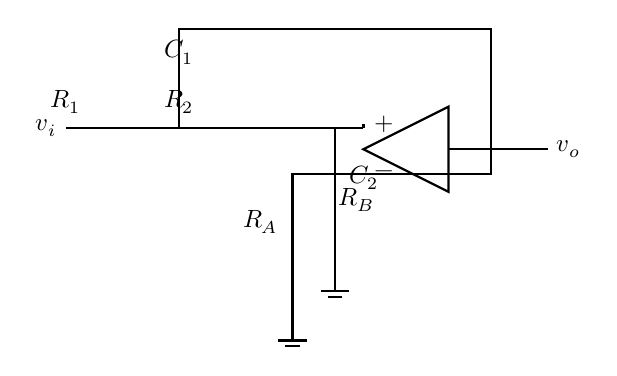
\begin{tikzpicture}[scale=0.9, transform shape]
  \draw[thick] (0, 0) node[left] {$v_i$} to[rectangle, draw=myteal, fill=hdrteal, minimum width=0.8cm, minimum height=0.4cm] (1.2, 0) node[midway, above=2pt] {$R_1$} -- (2.0, 0) to[rectangle, draw=myteal, fill=hdrteal, minimum width=0.8cm, minimum height=0.4cm] (3.2, 0) node[midway, above=2pt] {$R_2$} -- (4.2, 0);

  % Opamp
  \draw[thick] (4.2, -0.3) -- (5.4, 0.3) -- (5.4, -0.9) -- cycle;
  \node at (4.5, 0.05) {$+$}; \node at (4.5, -0.65) {$-$};
  \draw[thick] (4.2, 0) -- (4.2, 0.05);

  % Capacitor C2 to ground
  \draw[thick] (3.8, 0) -- (3.8, -1.4) to[rectangle, draw=myred, fill=hdrred, minimum width=0.7cm, minimum height=0.35cm] (3.8, -1.9) node[midway, right=2pt] {$C_2$} -- (3.8, -2.3);
  \draw[thick] (3.6, -2.3) -- (4.0, -2.3);
  \draw[thick] (3.7, -2.38) -- (3.9, -2.38);

  % Feedback Capacitor C1
  \draw[thick] (1.6, 0) -- (1.6, 1.4) to[rectangle, draw=myred, fill=hdrred, minimum width=0.7cm, minimum height=0.35cm] (3.8, 1.4) node[midway, above=2pt] {$C_1$} -- (6.0, 1.4) -- (6.0, -0.3);

  % Opamp output
  \draw[thick] (5.4, -0.3) -- (6.8, -0.3) node[right] {$v_o$};

  % Feedback resistors RA, RB
  \draw[thick] (4.2, -0.65) -- (3.2, -0.65) -- (3.2, -2.0) to[rectangle, draw=myteal, fill=hdrteal, minimum width=0.4cm, minimum height=0.7cm] (3.2, -2.7) node[midway, left=2pt] {$R_A$} -- (3.2, -3.0);
  \draw[thick] (3.0, -3.0) -- (3.4, -3.0);
  \draw[thick] (3.1, -3.08) -- (3.3, -3.08);
  \draw[thick] (3.2, -0.65) -- (5.0, -0.65) to[rectangle, draw=myteal, fill=hdrteal, minimum width=0.8cm, minimum height=0.4cm] (5.8, -0.65) node[midway, below=2pt] {$R_B$} -- (6.0, -0.65) -- (6.0, -0.3);
\end{tikzpicture}
\end{tcolorbox}

\begin{tcolorbox}[formulabox, title={2nd-Order Sallen-Key LPF Transfer Function and Design Equations}]
By applying Kirchhoff's Current Law at internal nodes:
\begin{equation}
  H(s) = \frac{v_o(s)}{v_i(s)} = \frac{A_F \omega_0^2}{s^2 + s \left(\frac{\omega_0}{Q}\right) + \omega_0^2}
\end{equation}
where:
\begin{equation}
  \omega_0 = \frac{1}{\sqrt{R_1 R_2 C_1 C_2}}, \qquad A_F = 1 + \frac{R_B}{R_A}
\end{equation}
For equal components $R_1 = R_2 = R$ and $C_1 = C_2 = C$:
\begin{equation}
  f_0 = \frac{1}{2\pi R C}, \qquad Q = \frac{1}{3 - A_F}
\end{equation}
\textbf{Butterworth Condition ($Q = 0.7071$)}:
\begin{equation}
  3 - A_F = \sqrt{2} \implies A_F = 3 - \sqrt{2} \approx 1.586 \implies \frac{R_B}{R_A} = 0.586
\end{equation}
Stopband roll-off is $-40\text{ dB/decade}$ ($-12\text{ dB/octave}$).
\end{tcolorbox}

\subsection{Second-Order Sallen-Key High-Pass Filter (HPF)}
Obtained by swapping the positions of resistors and capacitors in the Sallen-Key topology:
\begin{tcolorbox}[formulabox, title={2nd-Order Sallen-Key HPF Transfer Function}]
\begin{equation}
  H(s) = \frac{A_F s^2}{s^2 + s \left(\frac{\omega_0}{Q}\right) + \omega_0^2}
\end{equation}
with $f_0 = \frac{1}{2\pi R C}$ and $A_F = 1.586$ for maximally flat Butterworth response. Stopband attenuation rolls off at $+40\text{ dB/decade}$ below $f_0$.
\end{tcolorbox}

\subsection{Band-Pass and Band-Stop Filters}
\begin{itemize}[leftmargin=12pt, itemsep=3pt, topsep=2pt]
  \item \textbf{Multiple-Feedback (MFB) Band-Pass Filter}: Employs an inverting configuration with two feedback paths (one resistive, one capacitive). Provides stable, high-Q center frequency $f_0 = \frac{1}{2\pi C \sqrt{(R_1 \parallel R_2) R_3}}$.
  \item \textbf{Active Twin-T Notch Filter}: Rejects a single narrow frequency notch ($f_0 = \frac{1}{2\pi R C}$) while passing all other frequencies. Active bootstrapping via an op-amp follower sharpens the notch depth and increases the effective $Q$ factor up to 50.
\end{itemize}

% ─── Section 5: Quick Revision Page ───────────────────────────────────────────
\newpage
\section{Quick Revision Page}

\begin{tcolorbox}[formulabox, title={Key Formulas at a Glance}]
\begin{itemize}[leftmargin=12pt, itemsep=2pt, topsep=1pt]
  \item \textbf{Diff Amp Gain}: $A_d = -g_m R_C = -\frac{I_{EE} R_C}{2 V_T}$, \quad $A_c \approx -\frac{R_C}{2 R_E}$
  \item \textbf{Common Mode Rejection Ratio}: $\text{CMRR} = \left|\frac{A_d}{A_c}\right| \approx 2 g_m R_E = \frac{I_{EE} R_E}{V_T}$, \quad $\text{CMRR}_{\text{dB}} = 20\log_{10}(\text{CMRR})$
  \item \textbf{Input Common-Mode Range}: $V_{icm,\max} = V_{CC} - \frac{I_{EE}R_C}{2} + 0.7\text{ V}$, \quad $V_{icm,\min} = -V_{EE} + V_{CS} + 0.7\text{ V}$
  \item \textbf{Op-Amp Gain}: Inverting $A_v = -\frac{R_f}{R_1}$; \quad Non-Inverting $A_v = 1 + \frac{R_f}{R_1}$
  \item \textbf{Slew Rate \& Bandwidth}: $\text{SR} = \left.\frac{dv_o}{dt}\right|_{\max} = \frac{I_{EE}}{C_c}$, \quad $f_{\max} = \frac{\text{SR}}{2\pi V_m}$
  \item \textbf{Instrumentation Amp}: $v_o = \left(1 + \frac{2 R_1}{R_G}\right)\frac{R_3}{R_2}(v_2 - v_1)$
  \item \textbf{Lossy Integrator}: $H(s) = -\frac{R_f/R_1}{1 + s R_f C}$, \quad $f_a = \frac{1}{2\pi R_f C}$, \quad integration band $f \ge 10 f_a$
  \item \textbf{Schmitt Trigger Hysteresis}: $V_H = V_{UT} - V_{LT} = 2\,\frac{R_1}{R_1 + R_2} V_{sat}$
  \item \textbf{2nd-Order Sallen-Key LPF}: $f_0 = \frac{1}{2\pi RC}$, \quad Butterworth damping $A_F = 1.586$ ($Q = 0.707$)
\end{itemize}
\end{tcolorbox}

\begin{tcolorbox}[defbox, title={One-Line Definitions}]
\begin{itemize}[leftmargin=12pt, itemsep=2pt, topsep=1pt]
  \item \textbf{CMRR}: The ratio of differential voltage gain to common-mode voltage gain, expressing noise immunity.
  \item \textbf{Virtual Ground}: A node maintained at zero potential without being physically grounded, due to infinite open-loop gain.
  \item \textbf{Slew Rate}: The maximum rate of change of op-amp output voltage per unit time under large-signal step conditions.
  \item \textbf{Input Offset Voltage}: The differential DC voltage that must be applied between op-amp inputs to force output to zero.
  \item \textbf{Lossy Integrator}: An op-amp integrator with a shunt resistor across the feedback capacitor to clamp DC gain.
  \item \textbf{Schmitt Trigger}: A regenerative bi-stable comparator that utilizes positive feedback to create hysteresis.
  \item \textbf{Hysteresis}: The voltage separation between upper and lower switching thresholds that suppresses noise jitter.
  \item \textbf{Butterworth Filter}: An all-pole active filter exhibiting a maximally flat magnitude response in the passband.
\end{itemize}
\end{tcolorbox}

\begin{tcolorbox}[exambox, title={Frequently Asked / Viva Questions}]
\begin{enumerate}[leftmargin=14pt, itemsep=4pt, topsep=2pt]
  \item \Q{Why is an active current mirror preferred over a resistor in the emitter tail of a diff amp?}
  An active current mirror provides very high dynamic resistance ($r_o$ in M$\Omega$ range) while requiring negligible DC voltage drop, boosting CMRR to $> 100\text{ dB}$ without restricting supply rails.

  \item \Q{What causes the phenomenon of virtual ground in an op-amp circuit?}
  Since open-loop gain $A_{OL} \to \infty$ and output voltage $v_o$ is finite, the differential input voltage $v_d = v_+ - v_- = v_o / A_{OL} \to 0$. When $v_+$ is connected to ground ($0\text{ V}$), $v_-$ is forced to $0\text{ V}$.

  \item \Q{What is the primary drawback of an ideal op-amp integrator?}
  At DC ($\omega = 0$), capacitor impedance is infinite, causing the op-amp to run in open loop ($A_v \approx 10^5$). Tiny DC offset voltages saturate the output to the supply rail.

  \item \Q{How does a lossy integrator overcome output saturation?}
  By shunting a feedback resistor $R_f$ across capacitor $C$. At DC, the capacitor is open-circuit, setting a finite DC closed-loop gain $A_v(0) = -R_f/R_1$.

  \item \Q{What is the function of the level shifter stage inside an IC op-amp?}
  Because op-amp internal stages are direct-coupled, DC quiescent levels drift upwards toward $+V_{CC}$. The level shifter shifts the quiescent DC output level precisely to $0\text{ V}$.

  \item \Q{Why does a differentiator have stability issues at high frequencies?}
  Gain increases at $+20\text{ dB/decade}$ with frequency, amplifying high-frequency noise and introducing a $90^\circ$ phase lead that erodes phase margin, leading to spurious oscillation.

  \item \Q{Explain the role of hysteresis in a Schmitt trigger.}
  Hysteresis prevents high-frequency input noise from causing unwanted false transitions when the signal crosses the switching threshold.

  \item \Q{What is the 3-op-amp instrumentation amplifier's key advantage over a single op-amp diff amp?}
  Both inputs connect directly to non-inverting op-amp terminals, guaranteeing extremely high input impedance ($> 10^9\,\Omega$), while gain is tuned via a single floating resistor $R_G$.

  \item \Q{What condition must be satisfied for a 2nd-order Sallen-Key filter to achieve Butterworth response?}
  The quality factor must be $Q = 1/\sqrt{2} \approx 0.7071$, which dictates that passband gain $A_F = 3 - \sqrt{2} = 1.586$ ($R_B/R_A = 0.586$).

  \item \Q{What is Full-Power Bandwidth ($f_{\max}$)?}
  The maximum operating frequency at which an op-amp can deliver its rated maximum peak output voltage without experiencing slew-rate distortion: $f_{\max} = \frac{\text{SR}}{2\pi V_m}$.
\end{enumerate}
\end{tcolorbox}

\begin{tcolorbox}[tikzbox, title={Summary Comparison of Active Filter Topologies}]
\par\vspace{4pt}\noindent
\begin{tabularx}{\linewidth}{|B{3.2cm}|B{2.8cm}|B{2.8cm}|Y|}
\hline
\textbf{Filter Topology} & \textbf{Cutoff / Center Freq} & \textbf{Passband Gain} & \textbf{Key Features \& Trade-offs} \\
\hline
1st-Order Sallen-Key LPF & $f_c = \frac{1}{2\pi RC}$ & $A_F = 1 + \frac{R_f}{R_1}$ & $-20\text{ dB/dec}$ roll-off; simple, unconditionally stable. \\
\hline
2nd-Order Sallen-Key LPF & $f_0 = \frac{1}{2\pi RC}$ & $A_F = 1.586$ (Butterworth) & $-40\text{ dB/dec}$ roll-off; sharp knee; low component count. \\
\hline
2nd-Order Sallen-Key HPF & $f_0 = \frac{1}{2\pi RC}$ & $A_F = 1.586$ & $+40\text{ dB/dec}$ attenuation in stopband; high-pass filtering. \\
\hline
MFB Band-Pass Filter & $f_0 = \frac{1}{2\pi C \sqrt{R_{eq} R_3}}$ & $A_0 = -\frac{R_3}{2 R_1}$ & Inverting, stable high-$Q$ operation; low sensitivity to op-amp GBW. \\
\hline
Active Twin-T Notch & $f_0 = \frac{1}{2\pi RC}$ & Unity ($0\text{ dB}$) & High-$Q$ deep notch rejection; active bootstrap sharpens null depth. \\
\hline
\end{tabularx}
\end{tcolorbox}

\end{document}
